% 1991 年上海卷第 24 题：△ABC 与 △DBC 所在两平面互相垂直（依固定扫描页重绘，只画拓扑与标号，不按比例）
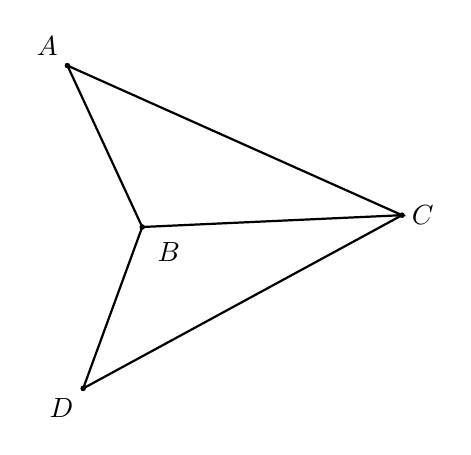
\begin{tikzpicture}[>=stealth,scale=1.0]
  \coordinate (B) at (0,0);
  \coordinate (C) at (3.3,0.15);
  \coordinate (A) at (-0.95,2.05);
  \coordinate (D) at (-0.75,-2.05);
  \draw[thick] (A)--(B)--(C)--cycle;
  \draw[thick] (B)--(D)--(C);
  \fill (A) circle (1pt) node[above left] {$A$};
  \fill (B) circle (1pt) node[below right=2pt] {$B$};
  \fill (C) circle (1pt) node[right] {$C$};
  \fill (D) circle (1pt) node[below left] {$D$};
\end{tikzpicture}
